% Options for packages loaded elsewhere
\PassOptionsToPackage{unicode}{hyperref}
\PassOptionsToPackage{hyphens}{url}
%
\documentclass[
]{article}
\usepackage{amsmath,amssymb}
\usepackage{lmodern}
\usepackage{iftex}
\ifPDFTeX
  \usepackage[T1]{fontenc}
  \usepackage[utf8]{inputenc}
  \usepackage{textcomp} % provide euro and other symbols
\else % if luatex or xetex
  \usepackage{unicode-math}
  \defaultfontfeatures{Scale=MatchLowercase}
  \defaultfontfeatures[\rmfamily]{Ligatures=TeX,Scale=1}
\fi
% Use upquote if available, for straight quotes in verbatim environments
\IfFileExists{upquote.sty}{\usepackage{upquote}}{}
\IfFileExists{microtype.sty}{% use microtype if available
  \usepackage[]{microtype}
  \UseMicrotypeSet[protrusion]{basicmath} % disable protrusion for tt fonts
}{}
\makeatletter
\@ifundefined{KOMAClassName}{% if non-KOMA class
  \IfFileExists{parskip.sty}{%
    \usepackage{parskip}
  }{% else
    \setlength{\parindent}{0pt}
    \setlength{\parskip}{6pt plus 2pt minus 1pt}}
}{% if KOMA class
  \KOMAoptions{parskip=half}}
\makeatother
\usepackage{xcolor}
\usepackage[margin=1in]{geometry}
\usepackage{color}
\usepackage{fancyvrb}
\newcommand{\VerbBar}{|}
\newcommand{\VERB}{\Verb[commandchars=\\\{\}]}
\DefineVerbatimEnvironment{Highlighting}{Verbatim}{commandchars=\\\{\}}
% Add ',fontsize=\small' for more characters per line
\usepackage{framed}
\definecolor{shadecolor}{RGB}{248,248,248}
\newenvironment{Shaded}{\begin{snugshade}}{\end{snugshade}}
\newcommand{\AlertTok}[1]{\textcolor[rgb]{0.94,0.16,0.16}{#1}}
\newcommand{\AnnotationTok}[1]{\textcolor[rgb]{0.56,0.35,0.01}{\textbf{\textit{#1}}}}
\newcommand{\AttributeTok}[1]{\textcolor[rgb]{0.77,0.63,0.00}{#1}}
\newcommand{\BaseNTok}[1]{\textcolor[rgb]{0.00,0.00,0.81}{#1}}
\newcommand{\BuiltInTok}[1]{#1}
\newcommand{\CharTok}[1]{\textcolor[rgb]{0.31,0.60,0.02}{#1}}
\newcommand{\CommentTok}[1]{\textcolor[rgb]{0.56,0.35,0.01}{\textit{#1}}}
\newcommand{\CommentVarTok}[1]{\textcolor[rgb]{0.56,0.35,0.01}{\textbf{\textit{#1}}}}
\newcommand{\ConstantTok}[1]{\textcolor[rgb]{0.00,0.00,0.00}{#1}}
\newcommand{\ControlFlowTok}[1]{\textcolor[rgb]{0.13,0.29,0.53}{\textbf{#1}}}
\newcommand{\DataTypeTok}[1]{\textcolor[rgb]{0.13,0.29,0.53}{#1}}
\newcommand{\DecValTok}[1]{\textcolor[rgb]{0.00,0.00,0.81}{#1}}
\newcommand{\DocumentationTok}[1]{\textcolor[rgb]{0.56,0.35,0.01}{\textbf{\textit{#1}}}}
\newcommand{\ErrorTok}[1]{\textcolor[rgb]{0.64,0.00,0.00}{\textbf{#1}}}
\newcommand{\ExtensionTok}[1]{#1}
\newcommand{\FloatTok}[1]{\textcolor[rgb]{0.00,0.00,0.81}{#1}}
\newcommand{\FunctionTok}[1]{\textcolor[rgb]{0.00,0.00,0.00}{#1}}
\newcommand{\ImportTok}[1]{#1}
\newcommand{\InformationTok}[1]{\textcolor[rgb]{0.56,0.35,0.01}{\textbf{\textit{#1}}}}
\newcommand{\KeywordTok}[1]{\textcolor[rgb]{0.13,0.29,0.53}{\textbf{#1}}}
\newcommand{\NormalTok}[1]{#1}
\newcommand{\OperatorTok}[1]{\textcolor[rgb]{0.81,0.36,0.00}{\textbf{#1}}}
\newcommand{\OtherTok}[1]{\textcolor[rgb]{0.56,0.35,0.01}{#1}}
\newcommand{\PreprocessorTok}[1]{\textcolor[rgb]{0.56,0.35,0.01}{\textit{#1}}}
\newcommand{\RegionMarkerTok}[1]{#1}
\newcommand{\SpecialCharTok}[1]{\textcolor[rgb]{0.00,0.00,0.00}{#1}}
\newcommand{\SpecialStringTok}[1]{\textcolor[rgb]{0.31,0.60,0.02}{#1}}
\newcommand{\StringTok}[1]{\textcolor[rgb]{0.31,0.60,0.02}{#1}}
\newcommand{\VariableTok}[1]{\textcolor[rgb]{0.00,0.00,0.00}{#1}}
\newcommand{\VerbatimStringTok}[1]{\textcolor[rgb]{0.31,0.60,0.02}{#1}}
\newcommand{\WarningTok}[1]{\textcolor[rgb]{0.56,0.35,0.01}{\textbf{\textit{#1}}}}
\usepackage{graphicx}
\makeatletter
\def\maxwidth{\ifdim\Gin@nat@width>\linewidth\linewidth\else\Gin@nat@width\fi}
\def\maxheight{\ifdim\Gin@nat@height>\textheight\textheight\else\Gin@nat@height\fi}
\makeatother
% Scale images if necessary, so that they will not overflow the page
% margins by default, and it is still possible to overwrite the defaults
% using explicit options in \includegraphics[width, height, ...]{}
\setkeys{Gin}{width=\maxwidth,height=\maxheight,keepaspectratio}
% Set default figure placement to htbp
\makeatletter
\def\fps@figure{htbp}
\makeatother
\setlength{\emergencystretch}{3em} % prevent overfull lines
\providecommand{\tightlist}{%
  \setlength{\itemsep}{0pt}\setlength{\parskip}{0pt}}
\setcounter{secnumdepth}{-\maxdimen} % remove section numbering
\ifLuaTeX
  \usepackage{selnolig}  % disable illegal ligatures
\fi
\IfFileExists{bookmark.sty}{\usepackage{bookmark}}{\usepackage{hyperref}}
\IfFileExists{xurl.sty}{\usepackage{xurl}}{} % add URL line breaks if available
\urlstyle{same} % disable monospaced font for URLs
\hypersetup{
  pdftitle={CI},
  pdfauthor={Niklas Pawelzik},
  hidelinks,
  pdfcreator={LaTeX via pandoc}}

\title{CI}
\author{Niklas Pawelzik}
\date{2023-05-18}

\begin{document}
\maketitle

\begin{Shaded}
\begin{Highlighting}[]
\FunctionTok{library}\NormalTok{(dagitty)}
\FunctionTok{library}\NormalTok{(ggdag)}
\end{Highlighting}
\end{Shaded}

\begin{verbatim}
## Warning: Paket 'ggdag' wurde unter R Version 4.2.3 erstellt
\end{verbatim}

\begin{verbatim}
## 
## Attache Paket: 'ggdag'
\end{verbatim}

\begin{verbatim}
## Das folgende Objekt ist maskiert 'package:stats':
## 
##     filter
\end{verbatim}

\begin{Shaded}
\begin{Highlighting}[]
\FunctionTok{library}\NormalTok{(ggplot2)}
\end{Highlighting}
\end{Shaded}

\hypertarget{high-level-dags}{%
\subsection{High Level DAGS}\label{high-level-dags}}

\begin{Shaded}
\begin{Highlighting}[]
\NormalTok{simplified\_assumed\_relationship }\OtherTok{\textless{}{-}} \FunctionTok{dagify}\NormalTok{(DID }\SpecialCharTok{\textasciitilde{}}\NormalTok{ HOD }\SpecialCharTok{+}\NormalTok{ RE }\SpecialCharTok{+}\NormalTok{ SE,}
\NormalTok{                                          NFNM }\SpecialCharTok{\textasciitilde{}}\NormalTok{ HOD }\SpecialCharTok{+}\NormalTok{ RE }\SpecialCharTok{+}\NormalTok{ SE,}
\NormalTok{                                          HOD }\SpecialCharTok{\textasciitilde{}}\NormalTok{ RE }\SpecialCharTok{+}\NormalTok{ SE }\SpecialCharTok{+}\NormalTok{ IF }\SpecialCharTok{+}\NormalTok{ OP }\SpecialCharTok{+}\NormalTok{ P }\SpecialCharTok{+}\NormalTok{ DC,}
\NormalTok{                                          RE }\SpecialCharTok{\textasciitilde{}}\NormalTok{ IF }\SpecialCharTok{+}\NormalTok{ SE,}
\NormalTok{                                          DC }\SpecialCharTok{\textasciitilde{}}\NormalTok{ OP }\SpecialCharTok{+}\NormalTok{ RE }\SpecialCharTok{+}\NormalTok{ IF, }\CommentTok{\# drug components other than heroin}
\NormalTok{                                          P }\SpecialCharTok{\textasciitilde{}}\NormalTok{ OP }\SpecialCharTok{+}\NormalTok{ RE }\SpecialCharTok{+}\NormalTok{ IF, }\CommentTok{\# purity/dose of heroin}
\NormalTok{                                          OP }\SpecialCharTok{\textasciitilde{}}\NormalTok{ L,}
                                          \AttributeTok{outcome =} \StringTok{"DID"}\NormalTok{,}
                                          \AttributeTok{exposure =} \StringTok{"OP"}\NormalTok{,}
                                          \AttributeTok{coords =} \FunctionTok{list}\NormalTok{(}\AttributeTok{x =} \FunctionTok{c}\NormalTok{(}\AttributeTok{L =} \SpecialCharTok{{-}}\DecValTok{2}\NormalTok{,}
                                                              \AttributeTok{OP =} \DecValTok{0}\NormalTok{,}
                                                              \AttributeTok{RE =} \DecValTok{4}\NormalTok{, }\AttributeTok{SE =} \DecValTok{6}\NormalTok{, }\AttributeTok{IF =} \DecValTok{2}\NormalTok{,}
                                                              \AttributeTok{P =} \FloatTok{2.67}\NormalTok{,}
                                                              \AttributeTok{DC =} \FloatTok{5.34}\NormalTok{,}
                                                              \AttributeTok{NFNM =} \DecValTok{10}\NormalTok{,}
                                                              \AttributeTok{HOD =} \DecValTok{8}\NormalTok{,}
                                                              \AttributeTok{DID =} \DecValTok{10}\NormalTok{), }
                                                        \AttributeTok{y =}  \FunctionTok{c}\NormalTok{(}\AttributeTok{L =} \DecValTok{0}\NormalTok{,}
                                                              \AttributeTok{OP =} \DecValTok{0}\NormalTok{,}
                                                              \AttributeTok{RE =} \DecValTok{4}\NormalTok{, }\AttributeTok{SE =} \DecValTok{5}\NormalTok{, }\AttributeTok{IF =} \DecValTok{3}\NormalTok{,}
                                                              \AttributeTok{P =} \DecValTok{1}\NormalTok{,}
                                                              \AttributeTok{DC =} \DecValTok{1}\NormalTok{,}
                                                              \AttributeTok{NFNM =} \DecValTok{1}\NormalTok{,}
                                                              \AttributeTok{HOD =} \DecValTok{0}\NormalTok{,}
                                                              \AttributeTok{DID =} \DecValTok{0}\NormalTok{)))}

\FunctionTok{ggdag\_status}\NormalTok{(simplified\_assumed\_relationship) }\SpecialCharTok{+}
  \FunctionTok{theme\_dag}\NormalTok{() }\SpecialCharTok{+}
  \FunctionTok{guides}\NormalTok{(}\AttributeTok{color =} \StringTok{"none"}\NormalTok{)}
\end{Highlighting}
\end{Shaded}

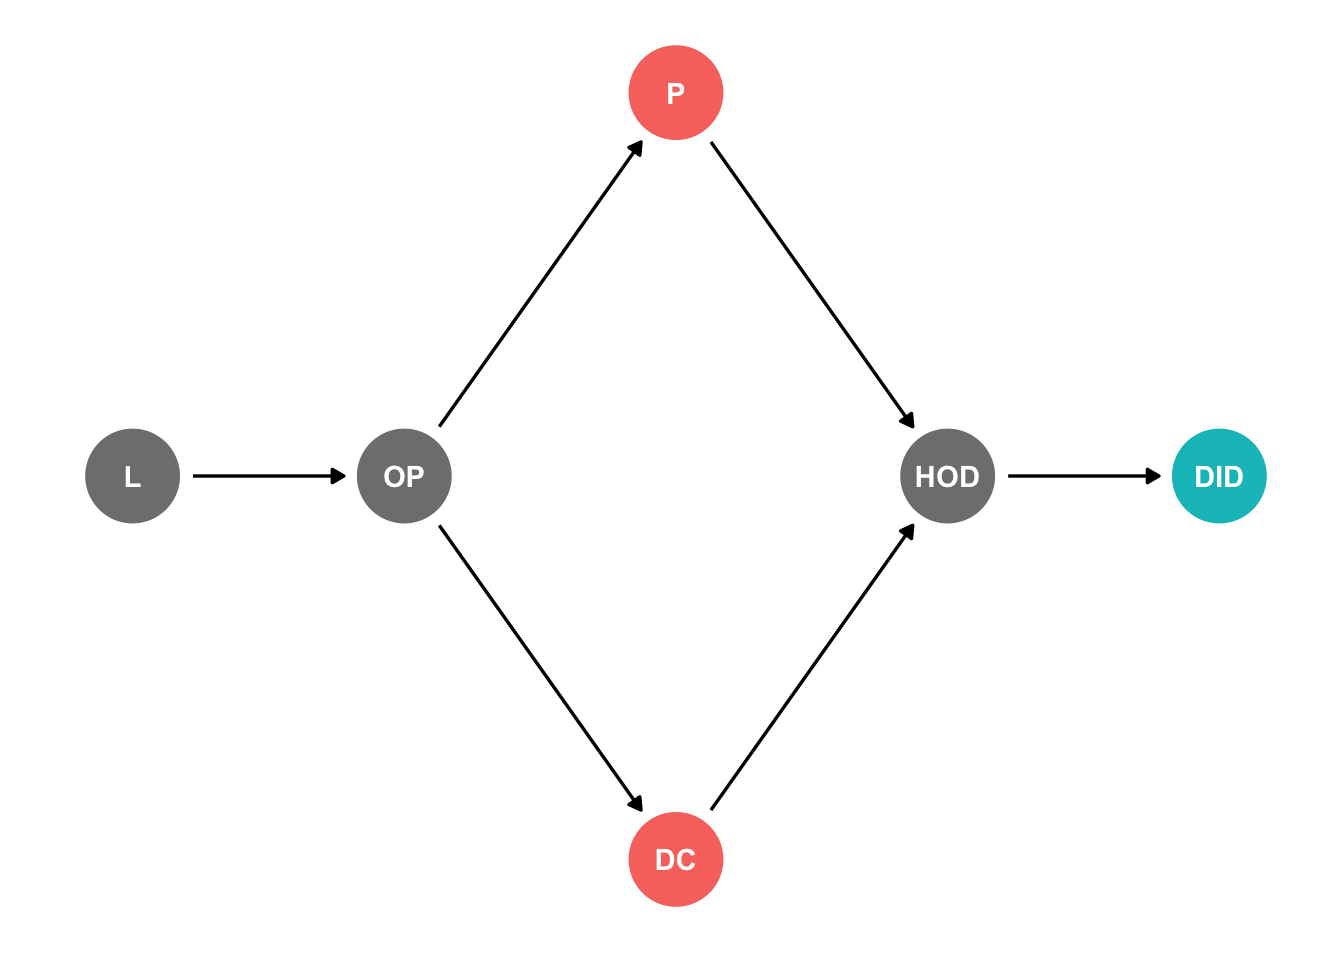
\includegraphics{DAGs_files/figure-latex/unnamed-chunk-2-1.pdf}

\begin{Shaded}
\begin{Highlighting}[]
\CommentTok{\# L = Legality}
\CommentTok{\# OP = Opioid Provision}
\CommentTok{\# RE = Risk Environment}
\CommentTok{\# SE = Social Environment}
\CommentTok{\# IF = Individual Factors}
\CommentTok{\# P = Purity}
\CommentTok{\# DC = Drug Components}
\CommentTok{\# NFNM = Non{-}Fatal Near Misses}
\CommentTok{\# HOD = Heroin Overdose}
\CommentTok{\# DID = Drug Induced Death }
\end{Highlighting}
\end{Shaded}

\hypertarget{proximal-causes-and-individual-factors}{%
\subsection{Proximal causes and individual
factors}\label{proximal-causes-and-individual-factors}}

``The proximal causes and individual factors associated with
heroin-related overdose (HOD) are well known {[}1,3,6,7{]}. Heroin
overdoses are frequently due to polydrug use (PDU), specifically when
heroin is combined with central nervous system depressants such as
alcohol and benzodiazepines that contribute to respiratory failure
{[}8{]}. A lack of experience (LOE) in heroin use and rapid changes in
tolerance due to incarceration (I), relapse following drug treatment (R)
or infrequent heroin use (IHU) have been linked to higher rates of
overdose {[}6,9--11{]}''

\begin{Shaded}
\begin{Highlighting}[]
\NormalTok{assumed\_relationship\_IF }\OtherTok{\textless{}{-}} \FunctionTok{dagify}\NormalTok{(DID }\SpecialCharTok{\textasciitilde{}}\NormalTok{ HOD }\SpecialCharTok{+}\NormalTok{ RE }\SpecialCharTok{+}\NormalTok{ SE,}
\NormalTok{                                          NFNM }\SpecialCharTok{\textasciitilde{}}\NormalTok{ HOD }\SpecialCharTok{+}\NormalTok{ RE }\SpecialCharTok{+}\NormalTok{ SE,}
\NormalTok{                                          HOD }\SpecialCharTok{\textasciitilde{}}\NormalTok{ RE }\SpecialCharTok{+}\NormalTok{ SE }\SpecialCharTok{+}\NormalTok{ PDU }\SpecialCharTok{+}\NormalTok{ LOE }\SpecialCharTok{+}\NormalTok{ I }\SpecialCharTok{+}\NormalTok{ IHU }\SpecialCharTok{+}\NormalTok{ R }\SpecialCharTok{+}\NormalTok{ OP }\SpecialCharTok{+}\NormalTok{ P }\SpecialCharTok{+}\NormalTok{ DC,}
\NormalTok{                                          RE }\SpecialCharTok{\textasciitilde{}}\NormalTok{ SE }\SpecialCharTok{+}\NormalTok{ PDU }\SpecialCharTok{+}\NormalTok{ LOE }\SpecialCharTok{+}\NormalTok{ I }\SpecialCharTok{+}\NormalTok{ IHU }\SpecialCharTok{+}\NormalTok{ R }\SpecialCharTok{+}\NormalTok{ OP }\SpecialCharTok{+}\NormalTok{ P }\SpecialCharTok{+}\NormalTok{ DC,}
\NormalTok{                                          DC }\SpecialCharTok{\textasciitilde{}}\NormalTok{ OP }\SpecialCharTok{+}\NormalTok{ RE }\SpecialCharTok{+}\NormalTok{ PDU }\SpecialCharTok{+}\NormalTok{ IHU }\SpecialCharTok{+}\NormalTok{ I }\SpecialCharTok{+}\NormalTok{ R, }\CommentTok{\# drug components other than heroin}
\NormalTok{                                          P }\SpecialCharTok{\textasciitilde{}}\NormalTok{ OP }\SpecialCharTok{+}\NormalTok{ RE }\SpecialCharTok{+}\NormalTok{ IHU }\SpecialCharTok{+}\NormalTok{ I }\SpecialCharTok{+}\NormalTok{ R, }\CommentTok{\# purity/dose of heroin}
\NormalTok{                                          OP }\SpecialCharTok{\textasciitilde{}}\NormalTok{ L,}
\NormalTok{                                          I }\SpecialCharTok{\textasciitilde{}}\NormalTok{ L,}
                                          \AttributeTok{outcome =} \StringTok{"DID"}\NormalTok{,}
                                          \AttributeTok{exposure =} \StringTok{"OP"}\NormalTok{,}
                                          \AttributeTok{latent =} \FunctionTok{c}\NormalTok{(}\StringTok{"PDU"}\NormalTok{, }\StringTok{"LOE"}\NormalTok{, }\StringTok{"I"}\NormalTok{, }\StringTok{"IHU"}\NormalTok{, }\StringTok{"R"}\NormalTok{), }\CommentTok{\# used to indicate Individual Factors}
                                          \AttributeTok{coords =} \FunctionTok{list}\NormalTok{(}\AttributeTok{x =} \FunctionTok{c}\NormalTok{(}\AttributeTok{L =} \SpecialCharTok{{-}}\DecValTok{2}\NormalTok{,}
                                                              \AttributeTok{OP =} \DecValTok{0}\NormalTok{,}
                                                              \AttributeTok{RE =} \DecValTok{4}\NormalTok{, }\AttributeTok{SE =} \DecValTok{6}\NormalTok{,}
                                                              \AttributeTok{I =} \DecValTok{1}\NormalTok{, }\AttributeTok{R =} \DecValTok{2}\NormalTok{, }\AttributeTok{PDU =} \DecValTok{3}\NormalTok{, }\AttributeTok{IHU =} \DecValTok{4}\NormalTok{, }\AttributeTok{LOE =} \DecValTok{5}\NormalTok{,}
                                                              \AttributeTok{P =} \FloatTok{2.67}\NormalTok{,}
                                                              \AttributeTok{DC =} \FloatTok{5.34}\NormalTok{,}
                                                              \AttributeTok{NFNM =} \DecValTok{10}\NormalTok{,}
                                                              \AttributeTok{HOD =} \DecValTok{8}\NormalTok{,}
                                                              \AttributeTok{DID =} \DecValTok{10}\NormalTok{), }
                                                        \AttributeTok{y =}  \FunctionTok{c}\NormalTok{(}\AttributeTok{L =} \DecValTok{0}\NormalTok{,}
                                                              \AttributeTok{OP =} \DecValTok{0}\NormalTok{,}
                                                              \AttributeTok{RE =} \DecValTok{4}\NormalTok{, }\AttributeTok{SE =} \DecValTok{5}\NormalTok{,}
                                                              \AttributeTok{I=} \SpecialCharTok{{-}}\DecValTok{1}\NormalTok{, }\AttributeTok{R =} \SpecialCharTok{{-}}\DecValTok{2}\NormalTok{, }\AttributeTok{PDU =} \SpecialCharTok{{-}}\DecValTok{3}\NormalTok{, }\AttributeTok{IHU =} \SpecialCharTok{{-}}\DecValTok{4}\NormalTok{, }\AttributeTok{LOE =} \SpecialCharTok{{-}}\DecValTok{5}\NormalTok{,}
                                                              \AttributeTok{P =} \DecValTok{1}\NormalTok{,}
                                                              \AttributeTok{DC =} \DecValTok{1}\NormalTok{,}
                                                              \AttributeTok{NFNM =} \DecValTok{1}\NormalTok{,}
                                                              \AttributeTok{HOD =} \DecValTok{0}\NormalTok{,}
                                                              \AttributeTok{DID =} \DecValTok{0}\NormalTok{)))}

\FunctionTok{ggdag\_status}\NormalTok{(assumed\_relationship\_IF) }\SpecialCharTok{+}
  \FunctionTok{theme\_dag}\NormalTok{() }\SpecialCharTok{+}
  \FunctionTok{guides}\NormalTok{(}\AttributeTok{color =} \StringTok{"none"}\NormalTok{)}
\end{Highlighting}
\end{Shaded}

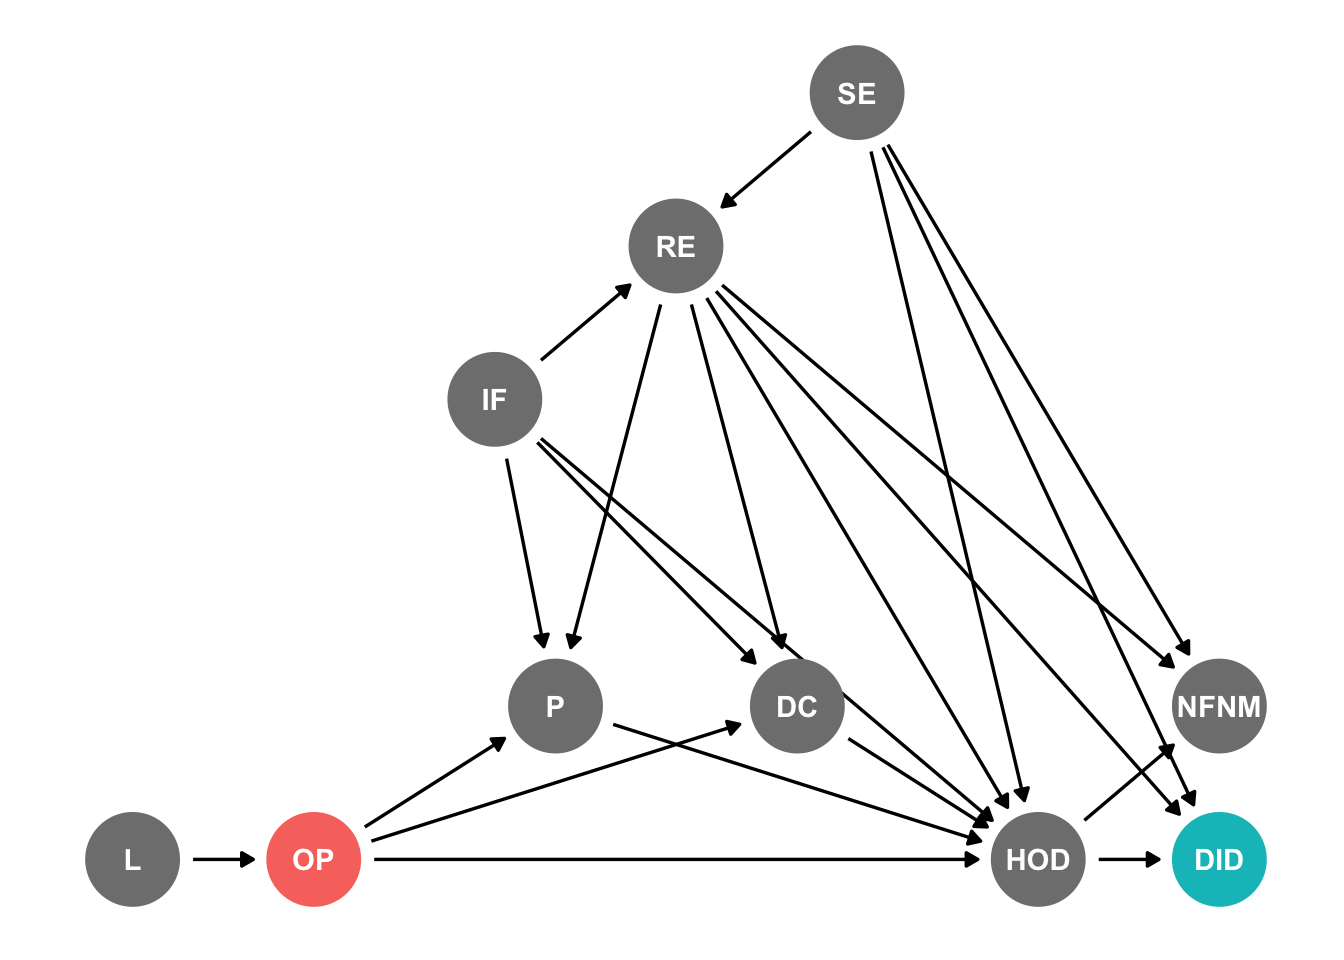
\includegraphics{DAGs_files/figure-latex/unnamed-chunk-3-1.pdf}

\begin{Shaded}
\begin{Highlighting}[]
\CommentTok{\# L = Legality}
\CommentTok{\# OP = Opioid Provision}
\CommentTok{\# RE = Risk Environment}
\CommentTok{\# SE = Social Environment}
\CommentTok{\# IF = Individual Factors}
\CommentTok{\# P = Purity}
\CommentTok{\# DC = Drug Components}
\CommentTok{\# NFNM = Non{-}Fatal Near Misses}
\CommentTok{\# HOD = Heroin Overdose}
\CommentTok{\# DID = Drug Induced Death }
\CommentTok{\# PDU = Polydrug Use}
\CommentTok{\# LOE = Lack of Experience}
\CommentTok{\# I = Incarceration}
\CommentTok{\# IHU = Infrequent Heroin Use}
\CommentTok{\# R = Relapse Following Drug Treatment}
\end{Highlighting}
\end{Shaded}

\hypertarget{social-causes}{%
\subsection{Social Causes}\label{social-causes}}

``Moving upstream, social causes such as poverty (EB), home-lessness
(HL), sexual minority status (SM) or other forms of social exclusion
(OSE) have also been linked to increased risk of drug overdose
{[}12--15{]}''

\begin{Shaded}
\begin{Highlighting}[]
\NormalTok{assumed\_relationship\_SC }\OtherTok{\textless{}{-}} \FunctionTok{dagify}\NormalTok{(DID }\SpecialCharTok{\textasciitilde{}}\NormalTok{ HOD }\SpecialCharTok{+}\NormalTok{ RE }\SpecialCharTok{+}\NormalTok{ HL }\SpecialCharTok{+}\NormalTok{ OSE,}
\NormalTok{                                          NFNM }\SpecialCharTok{\textasciitilde{}}\NormalTok{ HOD }\SpecialCharTok{+}\NormalTok{ RE,}
\NormalTok{                                          HOD }\SpecialCharTok{\textasciitilde{}}\NormalTok{ RE }\SpecialCharTok{+}\NormalTok{ IF }\SpecialCharTok{+}\NormalTok{ OP }\SpecialCharTok{+}\NormalTok{ P }\SpecialCharTok{+}\NormalTok{ DC }\SpecialCharTok{+}\NormalTok{ EB }\SpecialCharTok{+}\NormalTok{ HL }\SpecialCharTok{+}\NormalTok{ SM }\SpecialCharTok{+}\NormalTok{ OSE,}
\NormalTok{                                          RE }\SpecialCharTok{\textasciitilde{}}\NormalTok{ IF }\SpecialCharTok{+}\NormalTok{ HL }\SpecialCharTok{+}\NormalTok{ EB }\SpecialCharTok{+}\NormalTok{ SM }\SpecialCharTok{+}\NormalTok{ OSE,}
\NormalTok{                                          DC }\SpecialCharTok{\textasciitilde{}}\NormalTok{ OP }\SpecialCharTok{+}\NormalTok{ RE }\SpecialCharTok{+}\NormalTok{ IF, }\CommentTok{\# drug components other than heroin}
\NormalTok{                                          P }\SpecialCharTok{\textasciitilde{}}\NormalTok{ OP }\SpecialCharTok{+}\NormalTok{ RE }\SpecialCharTok{+}\NormalTok{ IF, }\CommentTok{\# purity/dose of heroin}
\NormalTok{                                          OP }\SpecialCharTok{\textasciitilde{}}\NormalTok{ L,}
\NormalTok{                                          HL }\SpecialCharTok{\textasciitilde{}}\NormalTok{ EB }\SpecialCharTok{+}\NormalTok{ SM }\SpecialCharTok{+}\NormalTok{ OSE }\SpecialCharTok{+}\NormalTok{ IF }\SpecialCharTok{+}\NormalTok{ HOD,}
\NormalTok{                                          EB }\SpecialCharTok{\textasciitilde{}}\NormalTok{ SM }\SpecialCharTok{+}\NormalTok{ OSE }\SpecialCharTok{+}\NormalTok{ IF,}
                                          \AttributeTok{outcome =} \StringTok{"DID"}\NormalTok{,}
                                          \AttributeTok{exposure =} \StringTok{"OP"}\NormalTok{,}
                                          \AttributeTok{latent =} \FunctionTok{c}\NormalTok{(}\StringTok{"EB"}\NormalTok{, }\StringTok{"HL"}\NormalTok{, }\StringTok{"SM"}\NormalTok{, }\StringTok{"OSE"}\NormalTok{),  }\CommentTok{\# used to indicate social environment}
                                          \AttributeTok{coords =} \FunctionTok{list}\NormalTok{(}\AttributeTok{x =} \FunctionTok{c}\NormalTok{(}\AttributeTok{L =} \SpecialCharTok{{-}}\DecValTok{2}\NormalTok{,}
                                                              \AttributeTok{OP =} \DecValTok{0}\NormalTok{,}
                                                              \AttributeTok{RE =} \DecValTok{4}\NormalTok{, }\AttributeTok{IF =} \DecValTok{2}\NormalTok{,}
                                                              \AttributeTok{EB =} \DecValTok{1}\NormalTok{, }\AttributeTok{HL =} \FloatTok{2.5}\NormalTok{,  }\AttributeTok{SM =} \DecValTok{3}\NormalTok{, }\AttributeTok{OSE =} \DecValTok{4}\NormalTok{,}
                                                              \AttributeTok{P =} \FloatTok{2.67}\NormalTok{,}
                                                              \AttributeTok{DC =} \FloatTok{5.34}\NormalTok{,}
                                                              \AttributeTok{NFNM =} \DecValTok{10}\NormalTok{,}
                                                              \AttributeTok{HOD =} \DecValTok{8}\NormalTok{,}
                                                              \AttributeTok{DID =} \DecValTok{10}\NormalTok{), }
                                                        \AttributeTok{y =}  \FunctionTok{c}\NormalTok{(}\AttributeTok{L =} \DecValTok{0}\NormalTok{,}
                                                              \AttributeTok{OP =} \DecValTok{0}\NormalTok{,}
                                                              \AttributeTok{RE =} \DecValTok{4}\NormalTok{, }\AttributeTok{IF =} \DecValTok{3}\NormalTok{,}
                                                              \AttributeTok{EB =} \SpecialCharTok{{-}}\DecValTok{1}\NormalTok{, }\AttributeTok{HL =} \SpecialCharTok{{-}}\DecValTok{2}\NormalTok{,  }\AttributeTok{SM =} \SpecialCharTok{{-}}\DecValTok{5}\NormalTok{, }\AttributeTok{OSE =} \SpecialCharTok{{-}}\DecValTok{8}\NormalTok{,}
                                                              \AttributeTok{P =} \DecValTok{1}\NormalTok{,}
                                                              \AttributeTok{DC =} \DecValTok{1}\NormalTok{,}
                                                              \AttributeTok{NFNM =} \DecValTok{1}\NormalTok{,}
                                                              \AttributeTok{HOD =} \DecValTok{0}\NormalTok{,}
                                                              \AttributeTok{DID =} \DecValTok{0}\NormalTok{)))}

\FunctionTok{ggdag\_status}\NormalTok{(assumed\_relationship\_SC) }\SpecialCharTok{+}
  \FunctionTok{theme\_dag}\NormalTok{() }\SpecialCharTok{+}
  \FunctionTok{guides}\NormalTok{(}\AttributeTok{color =} \StringTok{"none"}\NormalTok{)}
\end{Highlighting}
\end{Shaded}

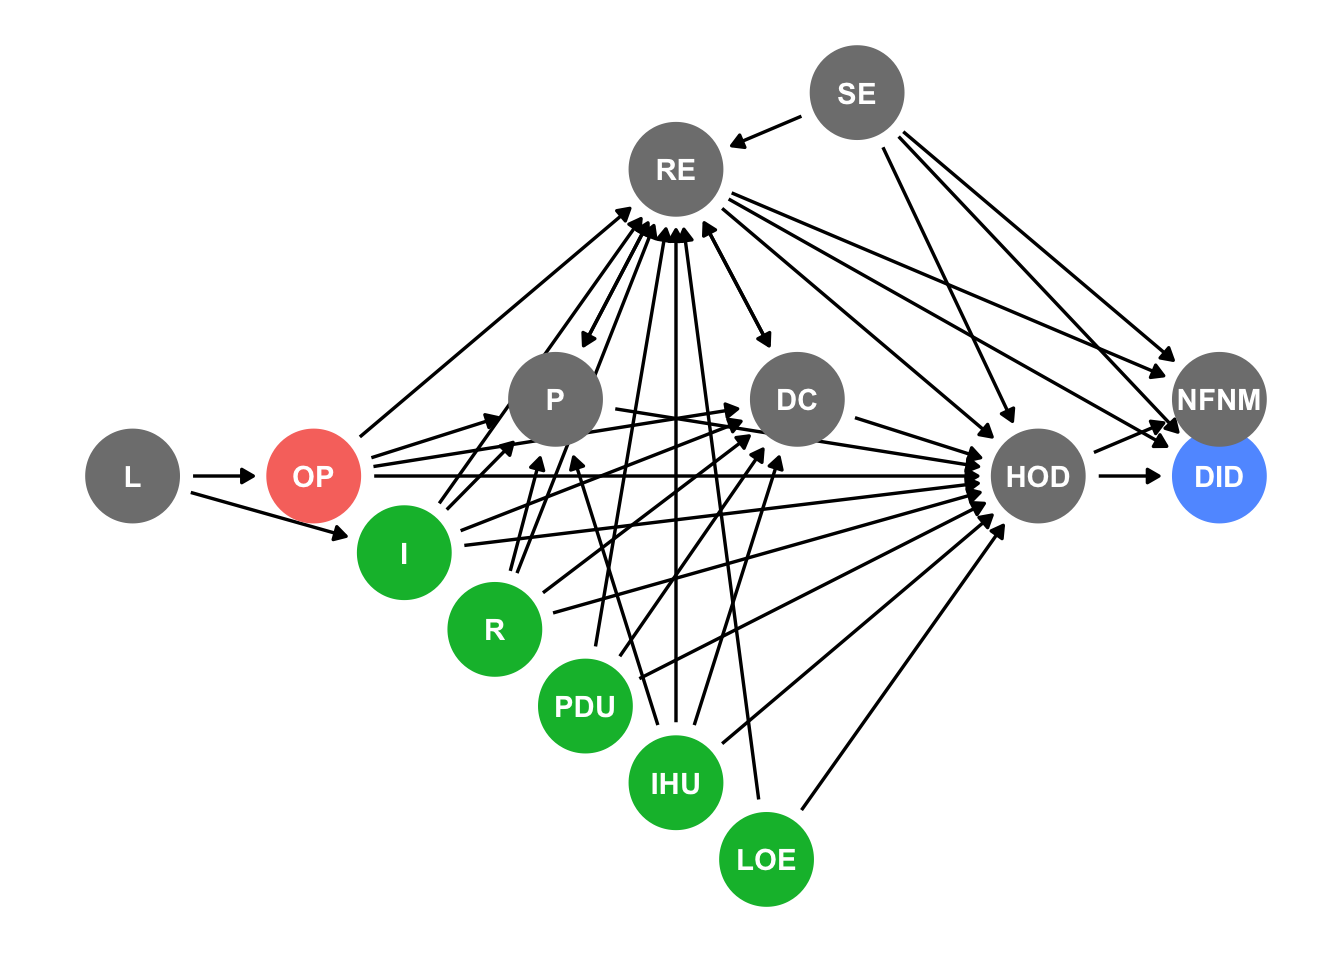
\includegraphics{DAGs_files/figure-latex/unnamed-chunk-4-1.pdf}

\begin{Shaded}
\begin{Highlighting}[]
\CommentTok{\# L = Legality}
\CommentTok{\# OP = Opioid Provision}
\CommentTok{\# RE = Risk Environment}
\CommentTok{\# SE = Social Environment}
\CommentTok{\# IF = Individual Factors}
\CommentTok{\# P = Purity}
\CommentTok{\# DC = Drug Components}
\CommentTok{\# NFNM = Non{-}Fatal Near Misses}
\CommentTok{\# HOD = Heroin Overdose}
\CommentTok{\# DID = Drug Induced Death }
\CommentTok{\# EB = Economic background}
\CommentTok{\# HL = Homelessness}
\CommentTok{\# SM = Sexual Minority Status}
\CommentTok{\# OSE = Other Forms of Social Exclusion}
\end{Highlighting}
\end{Shaded}

\hypertarget{risk-environment}{%
\subsection{Risk environment}\label{risk-environment}}

The risk environment represents a number of structural components that
moderate the relationship between individual factors and injection drug
users' (IDUs') health. For example, higher levels of drug law
enforcement (DLE) have been linked to increased risk of overdose deaths
{[}16{]}. The hypothesized agent of action is that increased criminal
justice risk (CJR) associated with drug use leads to specific behaviors,
e.g.~not calling for emergency help (i.e.~calling 911 in the United
States) following a witnessed overdose, which increase individual harm
associated with drug use {[}17{]}. Other structural factors such as
needle exchange (NE), naloxone distribution (ND), safe injection rooms
(SIR) and the availability of methadone treatment (MT) can reduce the
risk of overdose or harm associated with overdose in areas where these
services are available

\begin{Shaded}
\begin{Highlighting}[]
\NormalTok{assumed\_relationship\_RE }\OtherTok{\textless{}{-}} \FunctionTok{dagify}\NormalTok{(DID }\SpecialCharTok{\textasciitilde{}}\NormalTok{ HOD }\SpecialCharTok{+}\NormalTok{ SE }\SpecialCharTok{+}\NormalTok{ NE }\SpecialCharTok{+}\NormalTok{ SIR }\SpecialCharTok{+}\NormalTok{ ND,}
\NormalTok{                                          NFNM }\SpecialCharTok{\textasciitilde{}}\NormalTok{ HOD }\SpecialCharTok{+}\NormalTok{ SE }\SpecialCharTok{+}\NormalTok{ SIR }\SpecialCharTok{+}\NormalTok{ JCR }\SpecialCharTok{+}\NormalTok{ ND,}
\NormalTok{                                          HOD }\SpecialCharTok{\textasciitilde{}}\NormalTok{ SE }\SpecialCharTok{+}\NormalTok{ IF }\SpecialCharTok{+}\NormalTok{ OP }\SpecialCharTok{+}\NormalTok{ P }\SpecialCharTok{+}\NormalTok{ DC }\SpecialCharTok{+}\NormalTok{ SIR }\SpecialCharTok{+}\NormalTok{ NE }\SpecialCharTok{+}\NormalTok{ MT,}
\NormalTok{                                          RE }\SpecialCharTok{\textasciitilde{}}\NormalTok{ IF }\SpecialCharTok{+}\NormalTok{ JCR,}
\NormalTok{                                          JCR }\SpecialCharTok{\textasciitilde{}}\NormalTok{ DLE,}
\NormalTok{                                          DLE }\SpecialCharTok{\textasciitilde{}}\NormalTok{ L,}
\NormalTok{                                          DC }\SpecialCharTok{\textasciitilde{}}\NormalTok{ OP }\SpecialCharTok{+}\NormalTok{ SE }\SpecialCharTok{+}\NormalTok{ IF, }\CommentTok{\# drug components other than heroin}
\NormalTok{                                          P }\SpecialCharTok{\textasciitilde{}}\NormalTok{ OP }\SpecialCharTok{+}\NormalTok{ SE }\SpecialCharTok{+}\NormalTok{ IF, }\CommentTok{\# purity/dose of heroin}
\NormalTok{                                          OP }\SpecialCharTok{\textasciitilde{}}\NormalTok{ L,}
                                          \AttributeTok{latent =} \FunctionTok{c}\NormalTok{(}\StringTok{"DLE"}\NormalTok{, }\StringTok{"JCR"}\NormalTok{, }\StringTok{"NE"}\NormalTok{, }\StringTok{"ND"}\NormalTok{, }\StringTok{"SIR"}\NormalTok{, }\StringTok{"MT"}\NormalTok{), }\CommentTok{\# used to indicate risk environment}
                                          \AttributeTok{outcome =} \StringTok{"DID"}\NormalTok{,}
                                          \AttributeTok{exposure =} \StringTok{"OP"}\NormalTok{,}
                                          \AttributeTok{coords =} \FunctionTok{list}\NormalTok{(}\AttributeTok{x =} \FunctionTok{c}\NormalTok{(}\AttributeTok{L =} \SpecialCharTok{{-}}\DecValTok{2}\NormalTok{,}
                                                              \AttributeTok{OP =} \DecValTok{0}\NormalTok{,}
                                                              \AttributeTok{SE =} \DecValTok{6}\NormalTok{, }\AttributeTok{IF =} \DecValTok{2}\NormalTok{,}
                                                              \AttributeTok{DLE =} \DecValTok{1}\NormalTok{, }\AttributeTok{JCR =} \DecValTok{2}\NormalTok{, }\AttributeTok{NE =} \DecValTok{3}\NormalTok{, }\AttributeTok{ND =} \DecValTok{4}\NormalTok{, }\AttributeTok{SIR =} \DecValTok{5}\NormalTok{, }\AttributeTok{MT =} \DecValTok{6}\NormalTok{,}
                                                              \AttributeTok{P =} \FloatTok{2.67}\NormalTok{,}
                                                              \AttributeTok{DC =} \FloatTok{5.34}\NormalTok{,}
                                                              \AttributeTok{NFNM =} \DecValTok{10}\NormalTok{,}
                                                              \AttributeTok{HOD =} \DecValTok{8}\NormalTok{,}
                                                              \AttributeTok{DID =} \DecValTok{10}\NormalTok{), }
                                                        \AttributeTok{y =}  \FunctionTok{c}\NormalTok{(}\AttributeTok{L =} \DecValTok{0}\NormalTok{,}
                                                              \AttributeTok{OP =} \DecValTok{0}\NormalTok{,}
                                                              \AttributeTok{SE =} \DecValTok{4}\NormalTok{, }\AttributeTok{IF =} \DecValTok{3}\NormalTok{,}
                                                              \AttributeTok{DLE =} \SpecialCharTok{{-}}\DecValTok{1}\NormalTok{, }\AttributeTok{JCR =} \SpecialCharTok{{-}}\DecValTok{2}\NormalTok{, }\AttributeTok{NE =} \SpecialCharTok{{-}}\DecValTok{3}\NormalTok{, }\AttributeTok{ND =} \SpecialCharTok{{-}}\DecValTok{4}\NormalTok{, }\AttributeTok{SIR =} \SpecialCharTok{{-}}\DecValTok{5}\NormalTok{, }\AttributeTok{MT =} \SpecialCharTok{{-}}\DecValTok{6}\NormalTok{,}
                                                              \AttributeTok{P =} \DecValTok{1}\NormalTok{,}
                                                              \AttributeTok{DC =} \DecValTok{1}\NormalTok{,}
                                                              \AttributeTok{NFNM =} \DecValTok{1}\NormalTok{,}
                                                              \AttributeTok{HOD =} \DecValTok{0}\NormalTok{,}
                                                              \AttributeTok{DID =} \DecValTok{0}\NormalTok{)))}

\FunctionTok{ggdag\_status}\NormalTok{(assumed\_relationship\_RE) }\SpecialCharTok{+}
  \FunctionTok{theme\_dag}\NormalTok{() }\SpecialCharTok{+}
  \FunctionTok{guides}\NormalTok{(}\AttributeTok{color =} \StringTok{"none"}\NormalTok{)}
\end{Highlighting}
\end{Shaded}

\begin{verbatim}
## Warning: Removed 1 rows containing missing values (`geom_dag_point()`).
\end{verbatim}

\begin{verbatim}
## Warning: Removed 1 rows containing missing values (`geom_dag_text()`).
\end{verbatim}

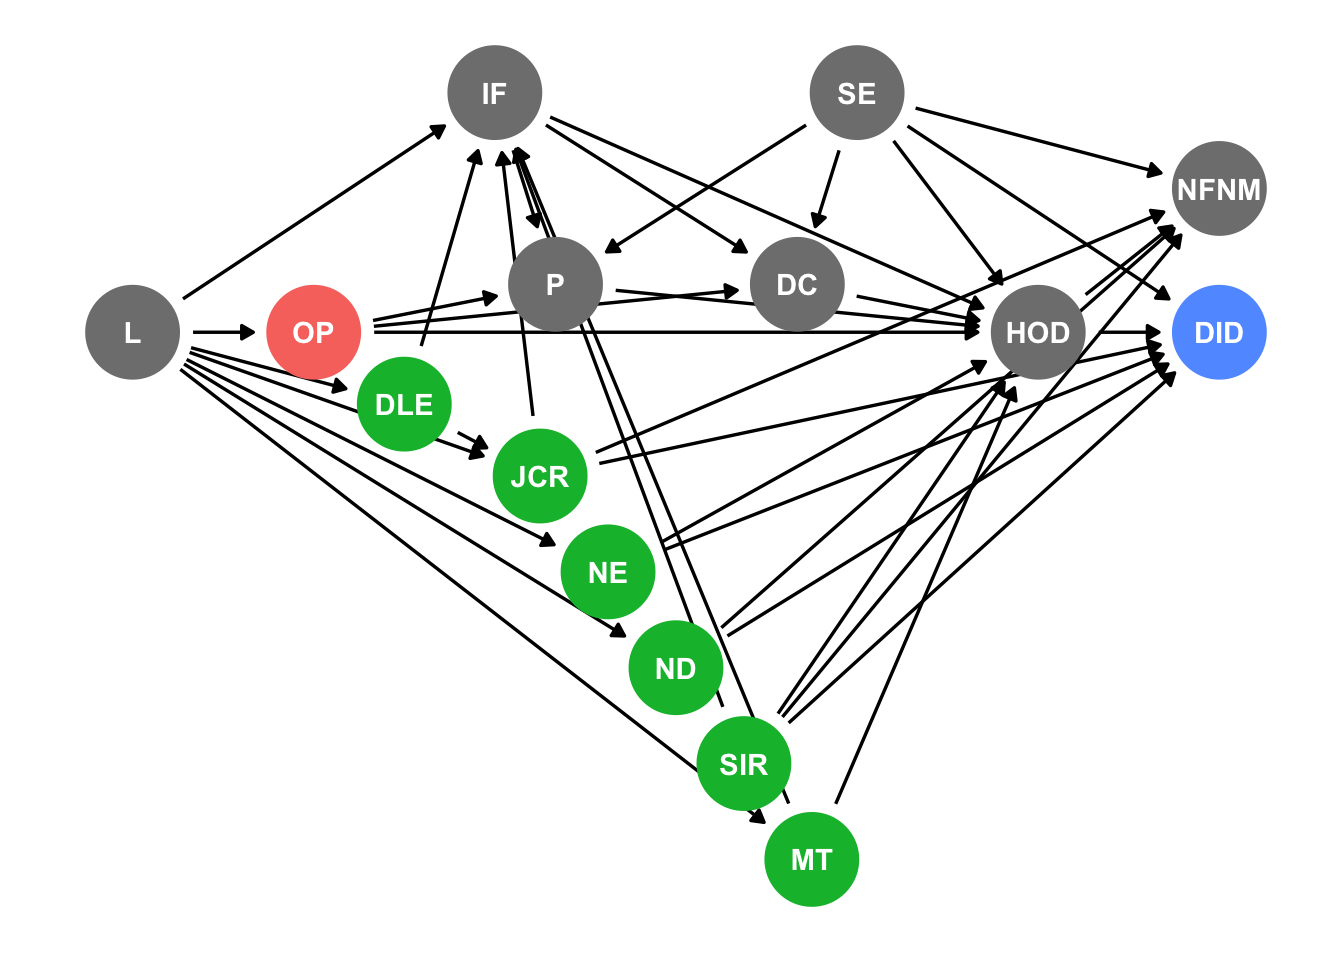
\includegraphics{DAGs_files/figure-latex/unnamed-chunk-5-1.pdf}

\begin{Shaded}
\begin{Highlighting}[]
\CommentTok{\# L = Legality}
\CommentTok{\# OP = Opioid Provision}
\CommentTok{\# RE = Risk Environment}
\CommentTok{\# SE = Social Environment}
\CommentTok{\# IF = Individual Factors}
\CommentTok{\# P = Purity}
\CommentTok{\# DC = Drug Components}
\CommentTok{\# NFNM = Non{-}Fatal Near Misses}
\CommentTok{\# HOD = Heroin Overdose}
\CommentTok{\# DID = Drug Induced Death }
\CommentTok{\# DLE = Drug Law Enforcement }
\CommentTok{\# CJR = Criminal justice risk}
\CommentTok{\# NE = Needle Exchange}
\CommentTok{\# ND = Naloxone Distribution}
\CommentTok{\# MT = Methadone Treatment }
\CommentTok{\# SIR = Safe Injection Rooms}
\end{Highlighting}
\end{Shaded}

\hypertarget{please-ignore-below}{%
\subsection{PLease ignore below}\label{please-ignore-below}}

\begin{Shaded}
\begin{Highlighting}[]
\CommentTok{\# PLEASE IGNORE!!}
\NormalTok{commonly\_assumed\_relationship }\OtherTok{\textless{}{-}} \FunctionTok{dagify}\NormalTok{(DID }\SpecialCharTok{\textasciitilde{}}\NormalTok{ HOD }\SpecialCharTok{+}\NormalTok{ CJR, }\CommentTok{\# drug induced death}
\NormalTok{                                  HOD }\SpecialCharTok{\textasciitilde{}}\NormalTok{ P }\SpecialCharTok{+}\NormalTok{ DC }\SpecialCharTok{+}\NormalTok{ PDU }\SpecialCharTok{+}\NormalTok{ LOE }\SpecialCharTok{+}\NormalTok{ I }\SpecialCharTok{+}\NormalTok{ IHU }\SpecialCharTok{+}\NormalTok{ R }\SpecialCharTok{+}
\NormalTok{                                        EB }\SpecialCharTok{+}\NormalTok{ HL }\SpecialCharTok{+}\NormalTok{ SM }\SpecialCharTok{+}\NormalTok{ OSE }\SpecialCharTok{+}\NormalTok{ SIR, }\CommentTok{\# heroin{-}related overdose}
\NormalTok{                                  DC }\SpecialCharTok{\textasciitilde{}}\NormalTok{ OP, }\CommentTok{\# drug components other than heroin}
\NormalTok{                                  P }\SpecialCharTok{\textasciitilde{}}\NormalTok{ OP }\SpecialCharTok{+}\NormalTok{ ND }\SpecialCharTok{+}\NormalTok{ NE, }\CommentTok{\# purity/dose of heroin}
\NormalTok{                                  NFNM }\SpecialCharTok{\textasciitilde{}}\NormalTok{ HOD, }\CommentTok{\# non{-}fatal near misses}
\NormalTok{                                  OP }\SpecialCharTok{\textasciitilde{}}\NormalTok{ L, }\CommentTok{\# legalization and opioid provision}
\NormalTok{                                  CJR }\SpecialCharTok{\textasciitilde{}}\NormalTok{ DLE,}
                        \AttributeTok{outcome =} \StringTok{"DID"}\NormalTok{,}
                        \CommentTok{\# latent = c("P", "OP"),}
                        \AttributeTok{exposure =} \StringTok{"OP"}\NormalTok{,}
                        \AttributeTok{coords =} \FunctionTok{list}\NormalTok{(}\AttributeTok{x =} \FunctionTok{c}\NormalTok{(}\AttributeTok{L =} \DecValTok{0}\NormalTok{,}
                                            \AttributeTok{DID =} \DecValTok{15}\NormalTok{, }\AttributeTok{HOD =} \DecValTok{13}\NormalTok{,}
                                            \AttributeTok{OP =} \DecValTok{1}\NormalTok{,  }\AttributeTok{P =} \DecValTok{2}\NormalTok{, }\AttributeTok{DC =} \DecValTok{2}\NormalTok{, }\AttributeTok{NFNM =} \DecValTok{15}\NormalTok{,}
                                            \AttributeTok{IHU =} \DecValTok{2}\NormalTok{, }\AttributeTok{R =} \DecValTok{3}\NormalTok{, }\AttributeTok{PDU =} \DecValTok{4}\NormalTok{, }\AttributeTok{LOE =} \DecValTok{5}\NormalTok{, }\AttributeTok{I =} \DecValTok{6}\NormalTok{, }
                                            \AttributeTok{EB =} \DecValTok{2}\NormalTok{, }\AttributeTok{HL =} \DecValTok{3}\NormalTok{,  }\AttributeTok{SM =} \DecValTok{4}\NormalTok{, }\AttributeTok{OSE =} \DecValTok{5}\NormalTok{,}
                                            \AttributeTok{DLE =} \DecValTok{5}\NormalTok{, }\AttributeTok{JCR =} \DecValTok{6}\NormalTok{, }\AttributeTok{NE =} \DecValTok{7}\NormalTok{, }\AttributeTok{ND =} \DecValTok{8}\NormalTok{, }\AttributeTok{SIR =} \DecValTok{9}\NormalTok{, }\AttributeTok{MT =} \DecValTok{4}\NormalTok{),}
                                      \AttributeTok{y =} \FunctionTok{c}\NormalTok{(}\AttributeTok{OP =} \DecValTok{1}\NormalTok{, }\AttributeTok{L =} \DecValTok{1}\NormalTok{, }\AttributeTok{DID =} \DecValTok{1}\NormalTok{, }\AttributeTok{HOD =} \DecValTok{1}\NormalTok{, }\AttributeTok{P =} \FloatTok{1.5}\NormalTok{, }\AttributeTok{DC =} \FloatTok{0.5}\NormalTok{, }\AttributeTok{NFNM =} \FloatTok{1.5}\NormalTok{, }\AttributeTok{PDU =} \DecValTok{2}\NormalTok{, }\AttributeTok{LOE =} \DecValTok{2}\NormalTok{, }\AttributeTok{I =} \DecValTok{2}\NormalTok{, }\AttributeTok{IHU =} \DecValTok{2}\NormalTok{, }\AttributeTok{R =} \DecValTok{2}\NormalTok{,}
                                            \AttributeTok{EB =} \DecValTok{0}\NormalTok{, }\AttributeTok{HL =} \DecValTok{0}\NormalTok{,  }\AttributeTok{SM =} \DecValTok{0}\NormalTok{, }\AttributeTok{OSE =} \DecValTok{0}\NormalTok{,}
                                            \AttributeTok{DLE =} \FloatTok{1.5}\NormalTok{, }\AttributeTok{JCR =} \FloatTok{1.5}\NormalTok{, }\AttributeTok{NE =} \FloatTok{1.5}\NormalTok{, }\AttributeTok{ND =} \FloatTok{1.5}\NormalTok{, }\AttributeTok{SIR =} \FloatTok{1.5}\NormalTok{, }\AttributeTok{MT =} \FloatTok{1.5}\NormalTok{)))}

\FunctionTok{ggdag\_status}\NormalTok{(commonly\_assumed\_relationship) }\SpecialCharTok{+}
  \FunctionTok{theme\_dag}\NormalTok{() }\SpecialCharTok{+}
  \FunctionTok{guides}\NormalTok{(}\AttributeTok{color =} \StringTok{"none"}\NormalTok{)  }\CommentTok{\# Turn off legend}
\end{Highlighting}
\end{Shaded}

\begin{verbatim}
## Warning: Removed 1 rows containing missing values (`geom_dag_point()`).
\end{verbatim}

\begin{verbatim}
## Warning: Removed 1 rows containing missing values (`geom_dag_text()`).
\end{verbatim}

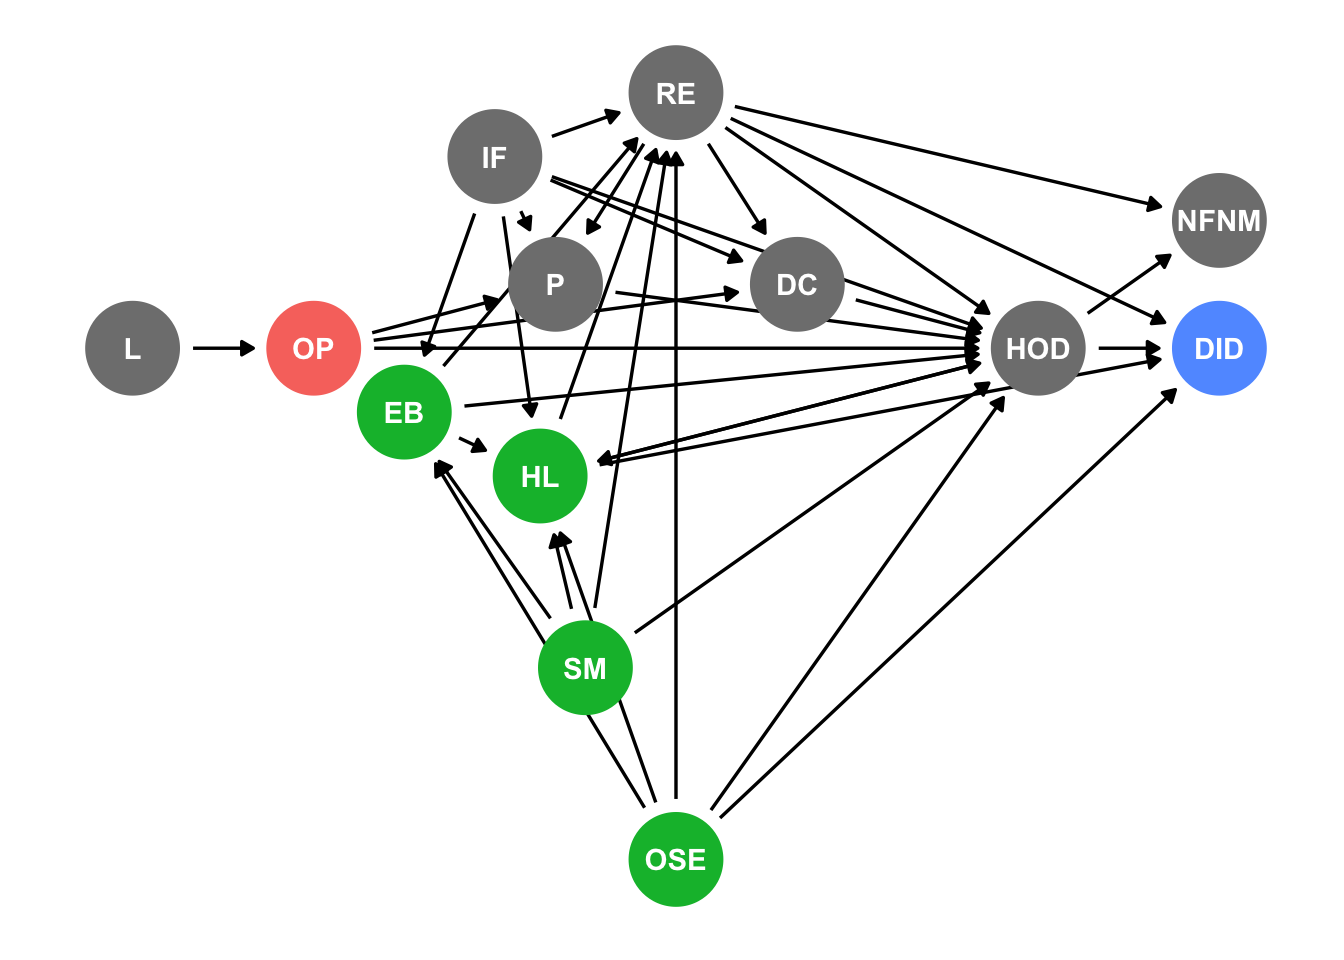
\includegraphics{DAGs_files/figure-latex/unnamed-chunk-6-1.pdf}

\hypertarget{including-plots}{%
\subsection{Including Plots}\label{including-plots}}

You can also embed plots, for example:

\includegraphics{DAGs_files/figure-latex/pressure-1.pdf}

Note that the \texttt{echo\ =\ FALSE} parameter was added to the code
chunk to prevent printing of the R code that generated the plot.

\end{document}
